% https://tex.stackexchange.com/q/742105/86
\documentclass[tikz,border=5pt]{standalone}
\usetikzlibrary{spath3}

\begin{document}

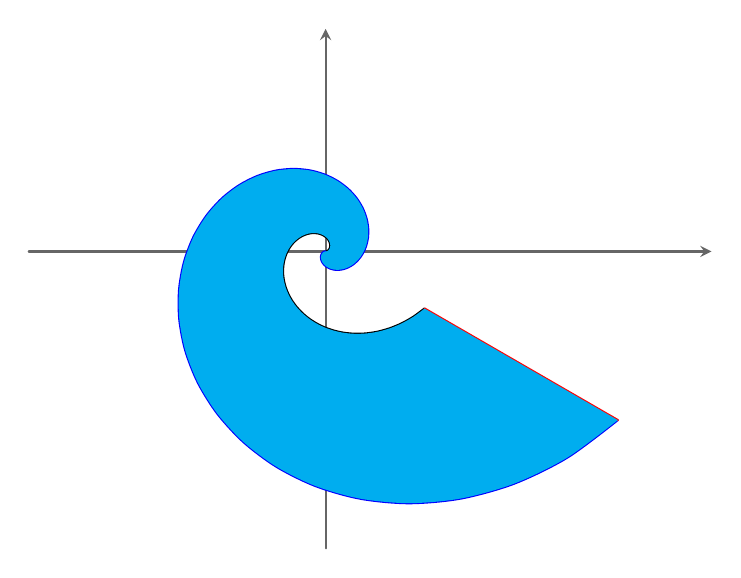
\begin{tikzpicture}[
    scale=0.3,>=stealth,
    x=1cm,y=1cm,
    line cap=round,
    line join=round,
]
% axes
\draw[->,color=black!60,line width=0.8] (-4*pi, 0) -- (5.2*pi, 0);
\draw[->,line width=0.8,color=black!60] (0, -4*pi) -- (0, 3*pi);
% inner spiral
\draw[
  spath/save=inner,%命名内部曲线
  smooth,black,thick,
  domain=0:11*pi/6,
  samples=50,%0,
  variable=\t
] plot ({deg(\t)}:{-1+((1+sqrt(5))/2)^(2*\t/pi)});
% outer spiral
\draw[
  spath/save=outer,%命名外部曲线
  smooth,blue,thick,
  domain=0:17*pi/6,
  samples=50,%0,
  variable=\t
] plot ({deg(\t)}:{1-((1+sqrt(5))/2)^(2*\t/pi)});
% joining line
\draw[
  spath/save=line,
  smooth,red,thick,
  domain=4.190109419:12.37110742,
  samples=10,%0,
  variable=\t
] plot ({\t}, {-1/sqrt(3)*\t});

% fill them by joining them together
\fill[
    cyan,
    spath/use=inner,
    spath/use={line,weld},
    spath/use={outer,weld,reverse},
];
\end{tikzpicture}

\end{document}